\documentclass{beamer}

\mode<presentation> {

% The Beamer class comes with a number of default slide themes
% which change the colors and layouts of slides. Below this is a list
% of all the themes, uncomment each in turn to see what they look like.

%\usetheme{default}
%\usetheme{AnnArbor}
%\usetheme{Antibes}
%\usetheme{Bergen}
%\usetheme{Berkeley}
%\usetheme{Berlin}
%\usetheme{Boadilla}
%\usetheme{CambridgeUS}
%\usetheme{Copenhagen}
%\usetheme{Darmstadt}
%\usetheme{Dresden}
%\usetheme{Frankfurt}
%\usetheme{Goettingen}
%\usetheme{Hannover}
%\usetheme{Ilmenau}
%\usetheme{JuanLesPins}
%\usetheme{Luebeck}
%\usetheme{Madrid}
%\usetheme{Malmoe}
%\usetheme{Marburg}
%\usetheme{Montpellier}
%\usetheme{PaloAlto}
%\usetheme{Pittsburgh}
%\usetheme{Rochester}
%\usetheme{Singapore}
%\usetheme{Szeged}
\usetheme{Warsaw}

% As well as themes, the Beamer class has a number of color themes
% for any slide theme. Uncomment each of these in turn to see how it
% changes the colors of your current slide theme.

%\usecolortheme{albatross}
%\usecolortheme{beaver}
%\usecolortheme{beetle}
%\usecolortheme{crane}
%\usecolortheme{dolphin}
%\usecolortheme{dove}
%\usecolortheme{fly}
%\usecolortheme{lily}
%\usecolortheme{orchid}
%\usecolortheme{rose}
%\usecolortheme{seagull}
%\usecolortheme{seahorse}
%\usecolortheme{whale}
%\usecolortheme{wolverine}

%\setbeamertemplate{footline} % To remove the footer line in all slides uncomment this line
%\setbeamertemplate{footline}[page number] % To replace the footer line in all slides with a simple slide count uncomment this line

%\setbeamertemplate{navigation symbols}{} % To remove the navigation symbols from the bottom of all slides uncomment this line
}

\usepackage{graphicx} % Allows including images
\usepackage{booktabs} % Allows the use of \toprule, \midrule and \bottomrule in tables

%----------------------------------------------------------------------------------------
%	TITLE PAGE
%----------------------------------------------------------------------------------------

\title{Sentiment Analysis of Twitter Feeds} % The short title appears at the bottom of every slide, the full title is only on the title page

\author[Yogesh Garg]{ % Short Name
Yogesh Garg\\ % Your name
\footnotesize{2009MT50635} % Your email address
} % Your name
\institute[IIT Delhi] % Your institution as it will appear on the bottom of every slide, may be shorthand to save space
{

\includegraphics[height=50pt]{img/iitd_logo.png}\\
Department of Mathematics\\
Indian Institute of Technology, Delhi \\ % Your institution for the title page
\medskip
%\footnotesize{2009MT50635} % Your email address
}
\date{\today} % Date, can be changed to a custom date

\begin{document}

\begin{frame}
\titlepage % Print the title page as the first slide
\end{frame}

\begin{frame}
\frametitle{Overview} % Table of contents slide, comment this block out to remove it
\tableofcontents % Throughout your presentation, if you choose to use \section{} and \subsection{} commands, these will automatically be printed on this slide as an overview of your presentation
\end{frame}

%----------------------------------------------------------------------------------------
%	PRESENTATION SLIDES
%----------------------------------------------------------------------------------------

%------------------------------------------------
\section{Introduction}
%------------------------------------------------

\begin{frame}
\frametitle{Introduction}
\begin{itemize}
\item User generated content on the web has two types
	\begin{itemize}
	\item Facts : Statements about topics
	\item Opinions : Display positive or negative sentiments
	\end{itemize}
\item Facts are easily collectible from the internet using search engines
		that index documents based on keywords
\item Opinionated texts are harder to categorise using keywords
\end{itemize}
Aim : 
\begin{itemize}
\item Identify and extract opinions expressed in Tweets using
		text analysis and natural language processing
\end{itemize}
\end{frame}

%------------------------------------------------
\subsection{Applications}
%------------------------------------------------

\begin{frame}
\frametitle{Applications}
\begin{description}
\item [Business] {Judge the market response of a product, intelligent placement of advertisments}
\item [Government] {Monitor public response to policies, issues raised during campaigns etc.}
\item [Finance] {Public opinion can be a good indicatior of a companies performance in the market}
\end{description}
\end{frame}

%------------------------------------------------
\subsection{Charachteristics}
%------------------------------------------------

\begin{frame}
\frametitle{Charachteristics of Tweets}
\begin{itemize}
\item Maximum length of a Twitter message is 140 characters
\item Use of colloquial language, slang, misspelings, hashtags
\item Tweets can be downloaded via Twitter API
\item Discussions often span across a variety of topics:
		Ideal for generics classifier
\end{itemize}

\begin{block}{Trivia}
Average length of a tweet is 14 words and 99 characters \\
There are aproximately 2 hashtags per tweet
\end{block}

\end{frame}

%------------------------------------------------
\section{Methodology}
\subsection{Datasets}
%------------------------------------------------

\begin{frame}
\frametitle{Datasets}

Twitter Sentiment Corpus
	\begin{itemize}
		\item 5513 hand annotated tweets
		\item 4 different topics: Apple, Google, Microsoft, and Twitter
		\item Each entry contains the tweet, sentiment, product, and query
		\item Downloaded using Twitter-Python open source library
	\end{itemize}

Stanford Twitter
	\begin{itemize}
		\item 100000 automatically annotated tweets
		\item Any tweet with positive emoticons were positive and vice-versa
	\end{itemize}

\begin{table}[h]
\centering
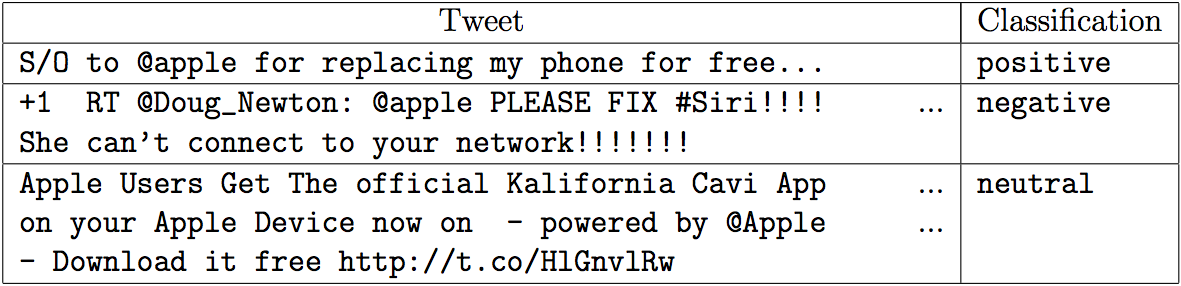
\includegraphics[width=0.8\textwidth]{img/table_tweets.png}
\caption{Classification of Tweets by sentiments expressed in each}
\label{table:twt}
\end{table}

\end{frame}

%------------------------------------------------
\subsection{Preprocessing}
%------------------------------------------------

\begin{frame}
\frametitle{Preprocessing}
\begin{itemize}
\item Required to normalize the text and decrease feature size
\end{itemize}
Steps:
\begin{itemize}
\item Remove product related query terms
\item Filter out URLs, Handles and Hashtags
\item Identify and replace emoticons
\item Filter a list of punctuations
\item Delete repeating charachters like, hurrrryyyy
\end{itemize}

\end{frame}

%------------------------------------------------

\begin{frame}
\frametitle{Preprocessing}
\begin{table}[h]
\centering
	\begin{tabular}{ l l l }
	\toprule
	\textbf{Step} & \textbf{Number} & \textbf{Percent}	\\
	\midrule
	before preprocessing & 19128 & \\
	\midrule
	after processing Hashtags & 18649 & 97.50\% \\
	after processing Handles & 17118 & 89.49\% \\
	after processing Urls & 16723 & 87.43\% \\
	after processing Emoticons & 18631 & 97.40\% \\
	after processing Punctuations & 13724 & 71.75\% \\
	after processing Repeatings & 18544 & 96.95\% \\
	\bottomrule
	after processing All & 11031 & 57.67\% \\
	\bottomrule
	\end{tabular}
\caption{Number of words before and after pre-processing}
\label{table:preproc_numwords}
\end{table}
\end{frame}

%------------------------------------------------

\begin{frame}
\frametitle{Features}

\begin{table}[h]
\centering
	\begin{tabular}{ l l l }
	\toprule
	\textbf{Feature    }& \textbf{Avg }& \textbf{Max }\\
	\midrule
	Handles    & 0.6761 & 8 \\
	Hashtags   & 2.028 & 13 \\
	Urls       & 0.4431 & 4 \\
	Emoticons  & 0.05500 & 3 \\
	\bottomrule
	\end{tabular}
\caption{Frequency of Features per Tweet}
\label{table:preproc_freq}
\end{table}

\end{frame}

%------------------------------------------------

\begin{frame}
\frametitle{Emoticons}
\begin{table}[h]
\centering
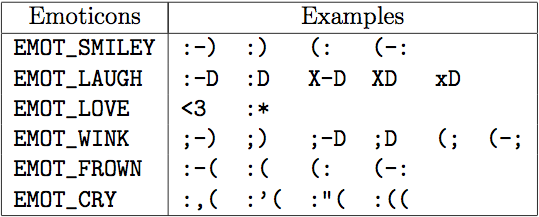
\includegraphics[scale=0.5]{img/table_emoticons.png}
\caption{List of Emoticons}
\label{table:emot}
\end{table}
\end{frame}

%------------------------------------------------

\begin{frame}
\frametitle{Punctuations}
\begin{table}[h]
\centering
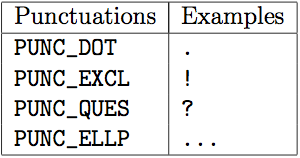
\includegraphics[scale=0.5]{img/table_punctuations.png}
\caption{List of Punctuations}
\label{table:punc}
\end{table}
\end{frame}

%------------------------------------------------
\subsection{Features}
%------------------------------------------------

\begin{frame}
\frametitle{Features}
\begin{itemize}
\item Word unigrams are the simplest features used in sentiment analysis
\item We train a Naive Bayes' Classifier trained on word unigrams
\item Investigated the relevance of word Bigrams and Trigrams
\end{itemize}
Other possible features include:
\begin{itemize}
\item Part-of-Speech tagging -- For each tweet, number of verbs, adverbs, adjectives, nouns etc are counted
\item Emoticons, Abbreviations, and intensifiers common on internet can be used to further improve the results
\end{itemize}

\end{frame}

%------------------------------------------------

\begin{frame}
\frametitle{Unigrams}

\begin{figure}[h]
\centering
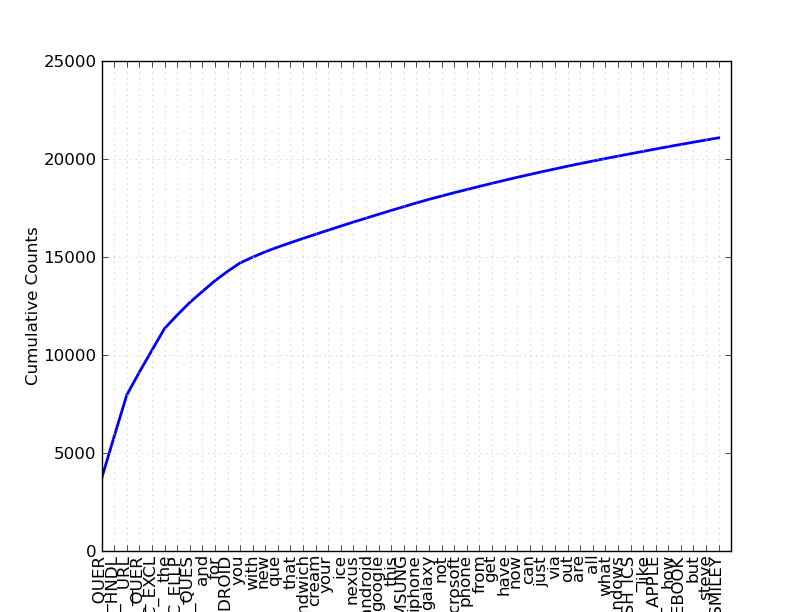
\includegraphics[width=0.75\textwidth]{img/fdist-unigrams.png}
\caption{Cumulative Frequency Plot for 50 Most Frequent Words}
\label{fig:unigrams}
\end{figure}

\end{frame}

%------------------------------------------------
\section{Experimentation}
%------------------------------------------------

\begin{frame}
\frametitle{Experimentation}
\begin{itemize}
\item A multi-class classifier to categorise a tweet into positive, negative or neutral
\item Trained using Naive Bayes model
\item We were able to get an accuracy of 83.92\%
\item Performance at par with baseline results discussed in papers
\end{itemize}
\end{frame}

%------------------------------------------------
\subsection{Naive Bayes Classifier}
%------------------------------------------------

\begin{frame}[fragile] % Need to use the fragile option when verbatim is used in the slide
\frametitle{Naive Bayes Classifier}

\begin{figure}[h]
\centering
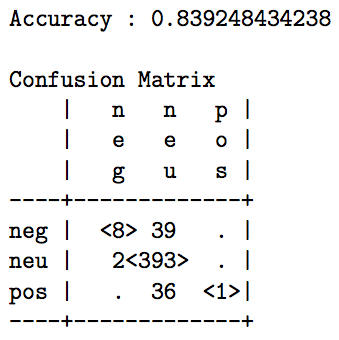
\includegraphics[scale=0.5]{img/fig_nb_stats.png}
\caption{Naive Bayes Statistics}
\label{fig:naive_accuracy}
\end{figure}

\end{frame}

%------------------------------------------------
\subsection{Best Classification Features}
%------------------------------------------------

\begin{frame}
\frametitle{Best Classification Features}
\begin{table}[h]
\centering
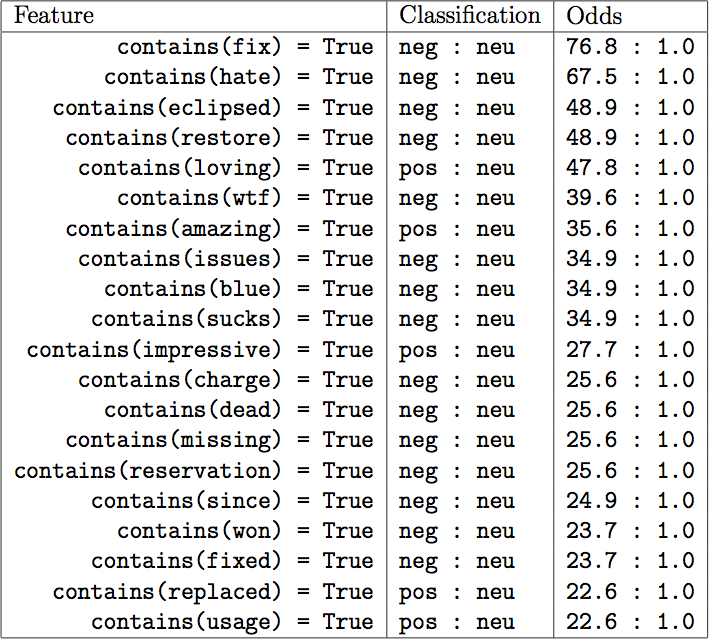
\includegraphics[scale=0.25]{img/table_bestfeatures.png}
\caption{Best Classification Features for Naive Bayes Classifier}
\label{table:naive_features}
\end{table}
\end{frame}

\begin{frame}
\frametitle{Best Classification Features}
\begin{table}[h]
\centering
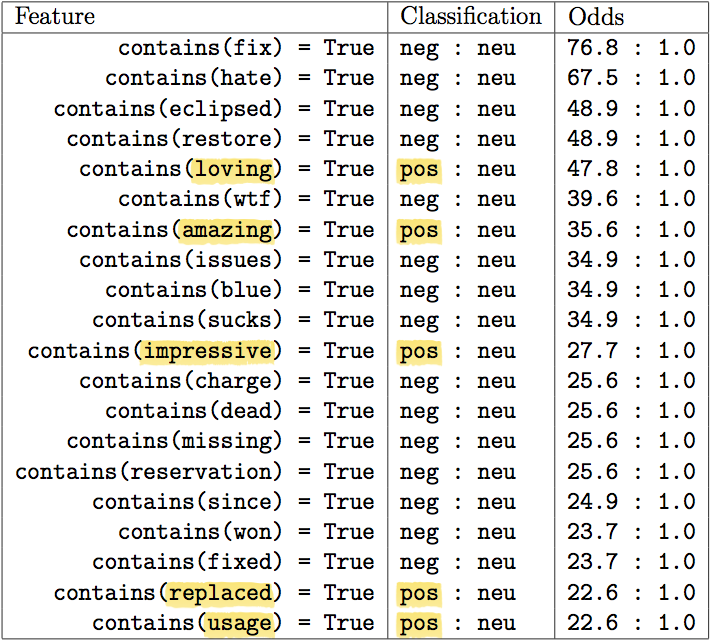
\includegraphics[scale=0.25]{img/table_bestfeatures_pos.png}
\caption{Best Classification Features for Naive Bayes Classifier}
\label{table:naive_features}
\end{table}
\end{frame}

\begin{frame}
\frametitle{Best Classification Features}
\begin{table}[h]
\centering
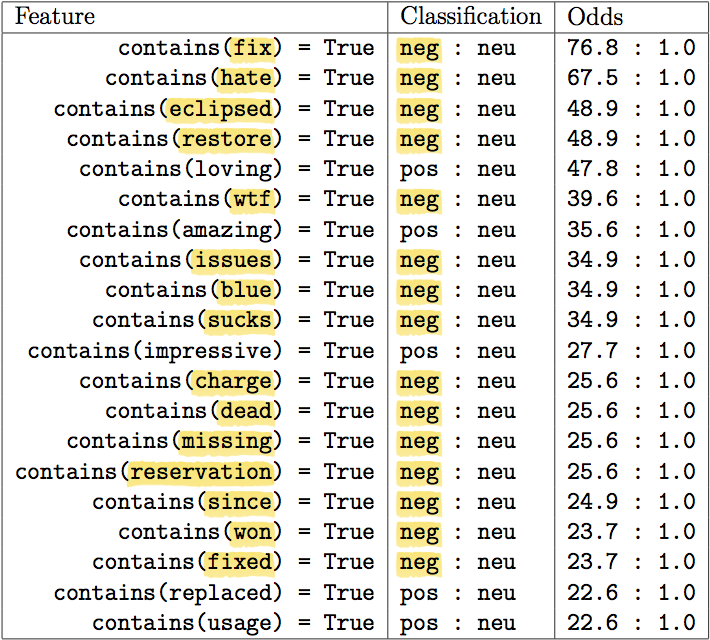
\includegraphics[scale=0.25]{img/table_bestfeatures_neg.png}
\caption{Best Classification Features for Naive Bayes Classifier}
\label{table:naive_features}
\end{table}
\end{frame}


%------------------------------------------------
\section{Conclusion}
\subsection{Results}
%------------------------------------------------

\begin{frame}
\frametitle{Results}
\begin{itemize}
\item Using relevant pre processing methods most important to improve the results considerably
\item The top classification features came out to be very relevant
\item We were able to get an accuracy of 83.92\%
\item Performance at par with baseline results discussed in papers
\end{itemize}

\begin{block}{Code}
The code for downloading the dataset, preprocessing and training the classifier
is made publicly available in an online repository:\\
\href{https://github.com/yogeshg/Twitter-Sentiment}
{\beamergotobutton{Link} github.com/yogeshg/Twitter-Sentiment}
\end{block}

\end{frame}
%------------------------------------------------
\subsection{Future Work}
%------------------------------------------------

\begin{frame}
\frametitle{Future Work}
\begin{itemize}
\item Use normalising techniques for imbalanced data
\item Two leveled classifier two classify into
		subjective or objective and then into, negative or positive
\item Also need to investigate performance on Maximum Entropy Classifier and Decision Trees
\end{itemize}
\end{frame}

%------------------------------------------------
\section*{Bibliography}
%------------------------------------------------

\begin{frame}
\frametitle{References}
\footnotesize{
\begin{thebibliography}{99} % Beamer does not support BibTeX so references must be inserted manually as below

%\bibitem[Smith, 2012]{p1} John Smith (2012)
%\newblock Title of the publication
%\newblock \emph{Journal Name} 12(3), 45 -- 678.

	\bibitem{survey}
				Bo Pang and Lillian Lee,
				``Opinion Mining and Sentiment Analysis''
				in \textit{Found. Trends Inf. Retr., 2(1-2)}:1–135.

	\bibitem{KWM}
				Efthymios Kouloumpis and Theresa Wilson and Johanna Moore,
				``Twitter Sentiment Analysis: The Good the Bad and the OMG!''
				in \textit{ICWSM, The AAAI Press}, (2011).

	\bibitem{PP}
				Alexander Pak and Patrick Paroubek,
				``Twitter as a Corpus for Sentiment Analysis and Opinion Mining''
				in \textit{Proceedings of the Seventh conference on International Language Resources and Evaluation LREC'10,
							Valletta, Malta, European Language Resources Association ELRA} (2010).

	\bibitem{SHA}
				Hassan Saif and Yulan He and Harith Alani,
				``Semantic Sentiment Analysis of Twitter''
				in \textit{The Semantic Web – ISWC} (2012).

\end{thebibliography}
}
\end{frame}

%------------------------------------------------

\begin{frame}
\frametitle{References}
\footnotesize{
\begin{thebibliography}{99} % Beamer does not support BibTeX so references must be inserted manually as below

%\bibitem[Smith, 2012]{p1} John Smith (2012)
%\newblock Title of the publication
%\newblock \emph{Journal Name} 12(3), 45 -- 678.

	\bibitem{S140}
				Alec Go and Richa Bhayani and Lei Huang,
				``Twitter Sentiment Classification using Distant Supervision''
				at Sentiment140, \textit{http://help.sentiment140.com/home} 
				in \textit{Processing} (2009).

	\bibitem{Pri}
				Balakrishnan Gokulakrishnan and Pavalanathan Priyanthan and
				Thiruchittampalam Ragavan and Nadarajah Prasath and AShehan Perera,
				``Opinion Mining and Sentiment Analysis on a Twitter Data Stream,''
				in \textit{The International Conference on Advances in ICT for Emerging Regions - ICTer} (2012).

	\bibitem{SA}
				Niek Sanders,
				\textit{http://www.sananalytics.com}

\end{thebibliography}
}
\end{frame}

%------------------------------------------------
\section*{The End}
%------------------------------------------------

\begin{frame}
\Huge{\centerline{Questions and Suggestions?}}
\end{frame}
%------------------------------------------------

\begin{frame}
\Huge{\centerline{Thanks}}
\end{frame}

%----------------------------------------------------------------------------------------

\end{document} 